\PassOptionsToPackage{unicode=true}{hyperref} % options for packages loaded elsewhere
\PassOptionsToPackage{hyphens}{url}
%
\documentclass[10pt,a4paper,]{article}
\usepackage{lmodern}
\usepackage{amssymb,amsmath}
\usepackage{ifxetex,ifluatex}
\usepackage{fixltx2e} % provides \textsubscript
\ifnum 0\ifxetex 1\fi\ifluatex 1\fi=0 % if pdftex
  \usepackage[T1]{fontenc}
  \usepackage[utf8]{inputenc}
  \usepackage{textcomp} % provides euro and other symbols
\else % if luatex or xelatex
  \usepackage{unicode-math}
  \defaultfontfeatures{Ligatures=TeX,Scale=MatchLowercase}
\fi
% use upquote if available, for straight quotes in verbatim environments
\IfFileExists{upquote.sty}{\usepackage{upquote}}{}
% use microtype if available
\IfFileExists{microtype.sty}{%
\usepackage[]{microtype}
\UseMicrotypeSet[protrusion]{basicmath} % disable protrusion for tt fonts
}{}
\usepackage{hyperref}
\hypersetup{
            pdftitle={PL0 Static Semantics Cheat Sheet},
            pdfauthor={Kenton Lam},
            pdfborder={0 0 0},
            breaklinks=true}
\urlstyle{same}  % don't use monospace font for urls
\usepackage{graphicx,grffile}
\makeatletter
\def\maxwidth{\ifdim\Gin@nat@width>\linewidth\linewidth\else\Gin@nat@width\fi}
\def\maxheight{\ifdim\Gin@nat@height>\textheight\textheight\else\Gin@nat@height\fi}
\makeatother
% Scale images if necessary, so that they will not overflow the page
% margins by default, and it is still possible to overwrite the defaults
% using explicit options in \includegraphics[width, height, ...]{}
\setkeys{Gin}{width=\maxwidth,height=\maxheight,keepaspectratio}
\setlength{\emergencystretch}{3em}  % prevent overfull lines
\providecommand{\tightlist}{%
  \setlength{\itemsep}{0pt}\setlength{\parskip}{0pt}}
\setcounter{secnumdepth}{0}
% Redefines (sub)paragraphs to behave more like sections
\ifx\paragraph\undefined\else
\let\oldparagraph\paragraph
\renewcommand{\paragraph}[1]{\oldparagraph{#1}\mbox{}}
\fi
\ifx\subparagraph\undefined\else
\let\oldsubparagraph\subparagraph
\renewcommand{\subparagraph}[1]{\oldsubparagraph{#1}\mbox{}}
\fi

% set default figure placement to htbp
\makeatletter
\def\fps@figure{htbp}
\makeatother


\title{PL0 Static Semantics Cheat Sheet}
\author{Kenton Lam}
\date{Friday July 3, 2020}

\begin{document}
\maketitle

\begin{abstract}
  A quick reference on static semantics of the PL0 programming language.
This is meant to be read alongside \texttt{PL0-SSemantics.pdf}. Written
by Kenton Lam.
\end{abstract}

\hypertarget{abstract-syntax}{%
\subsection{Abstract Syntax}\label{abstract-syntax}}


\includegraphics[width=0.5\textwidth]{assets/image-20200703170905035.png}

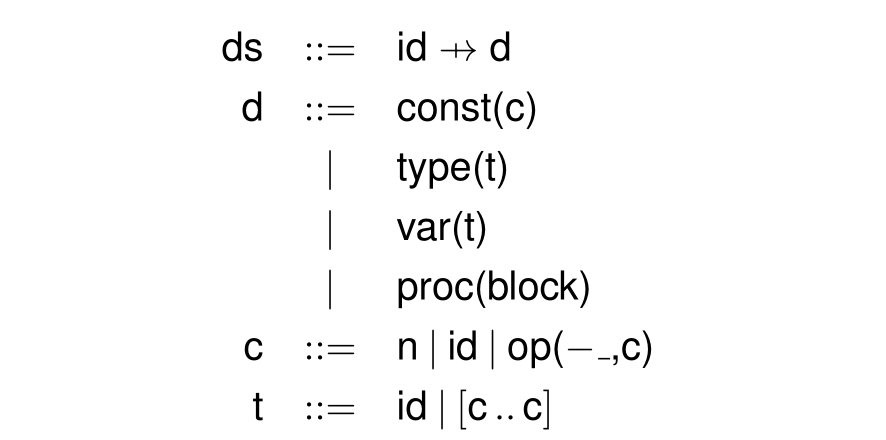
\includegraphics[width=0.5\textwidth]{assets/image-20200703170927076.png}

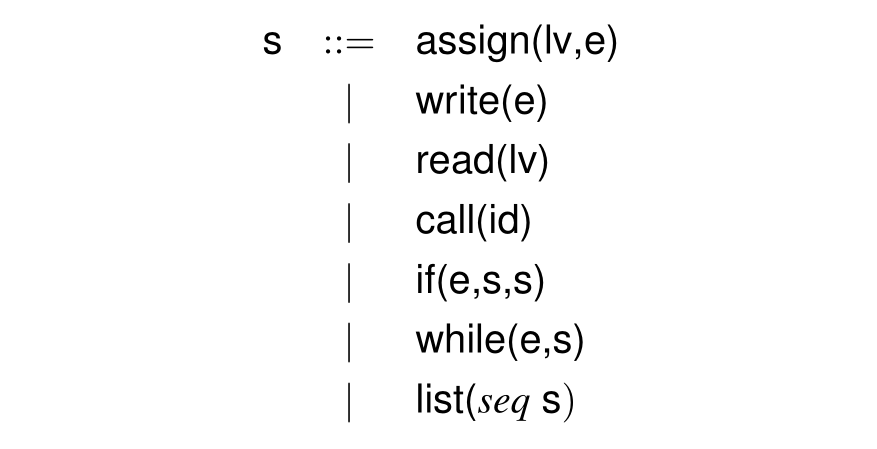
\includegraphics[width=0.5\textwidth]{assets/image-20200703170959717.png}

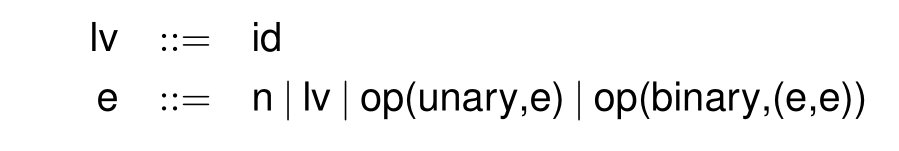
\includegraphics[width=0.5\textwidth]{assets/image-20200703171012542.png}

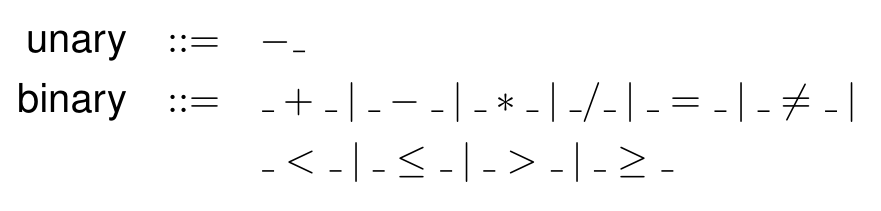
\includegraphics[width=0.5\textwidth]{assets/image-20200703171023633.png}


\hypertarget{notation}{%
\subsection{Notation}\label{notation}}

\begin{itemize}
\tightlist
\item
  Abstract syntax is written in sans-serif font. For example the
  expression \texttt{y+1} in code is written as \(\textsf {y} + 1\)
  here. This corresponds to expression nodes and statement nodes.
\item
  Semantic constructs are written in \(\textit{italics}\). For example,
  the type \(\operatorname{\textit{ref}}\,(T)\). These are most commonly
  types or other static checker constructs like the symbol table.
\item
  The use of arrows is very precise:

  \begin{itemize}
  \tightlist
  \item
    \(\to\) denotes functions,
  \item
    \(\mapsto\) denotes mapping values,
  \item
    \(\overset e\to\) denotes evaluates to, and
  \item
    \(\to\) with a vertical line in the centre denotes a mapping type
    (we will use \(\twoheadrightarrow\) here because I can't type it).
  \end{itemize}
\item
  A bullet \(\bullet\) is used to separate quantifiers from their
  predicate.
\item
  \(=\) denotes equivalence in the mathematical sense (a strong
  statement).
\end{itemize}

With the above in mind, we define a few more high-level pieces.

\begin{itemize}
\item
  A mapping \(M\) of \(a \twoheadrightarrow b\) has some operations
  defined:

  \begin{itemize}
  \tightlist
  \item
    \(\operatorname*{dom}(M)\) returns the set of \(a\) keys in the
    mapping,
  \item
    \(M(a)\) returns the \(b\) value mapped to by the key \(a\), and
  \item
    \(M_1 \oplus M_2\) returns a mapping containing the entries of both
    \(M_1\) and \(M_2\), with entries in \(M_2\) overriding \(M_1\) if
    both are present.
  \end{itemize}
\item
  \(\textit{syms}\) is defined as a mapping
  \(\textsf{id} \twoheadrightarrow \textit{SymEntry}\) of AST
  identifiers to symbol table entries, so
  \(\operatorname*{dom}(\textit{syms})\) is the set of defined
  identifiers. A symbol table entry is a sum type defined as \[
  \begin{aligned}
  \textit{SymEntry} &::= \textit{ConstEntry}(T, \mathbb Z) \mid \textit{TypeEntry}(T) \\
  &\qquad\mid \textit{VarEntry}(T) \mid \textit{ProcEntry}(\textsf{block}).
  \end{aligned}
  \]
\item
  \(\textit{syms} \vdash \textsf e : T\) means in the context of the
  symbol table \(\textit{syms}\), the expression \(\textsf e\) is
  well-typed and has the type \(T\).
\end{itemize}

\hypertarget{declarations}{%
\subsection{Declarations}\label{declarations}}

There are four forms of declarations: constants, types, variables, and
procedures. The notation
\(\textit{syms} \vdash \textit{WFDeclaration}(\textsf d)\) means that
\(\textsf d\) is a well-formed declaration in the context of
\(\textit{syms}\). Furthermore, \[
\textit{entry}(\textit{syms}, \textsf d)=\textit{ent}
\] is used to assign \(\textit{ent}\) to the symbol table entry of
\(\textsf d\). This formally assigns a SymEntry to a particular
declaration form \(\textsf{d}\). Perhaps more rigorously, the statement
\[
\textit{entry}(\textit{syms}, \textsf{var}(\textsf{t})) = \textit{VarEntry}(\textit{ref}(T))
\] means that a declaration of the form \(\textsf{var}(\textsf{t})\)
should have a corresponding VarEntry table when interpreted in the
context of \(\textit{syms}\).

The declaration rules use pattern matching in their consequents, which
means only expressions of a certain form can be well-formed
declarations. This prevents us from declaring a type of, say, \(1+10\).

\hypertarget{types}{%
\subsection{Types}\label{types}}

These rules concern the definition of types in PL0 program (e.g.~type
aliases and subrange types).

We introduce a function \(\textit{typeof}\) such that
\(\textit{typeof}(\textsf{e}) =T\) means the given expression
\textbf{is} (i.e.~defines) the type \(T\). This is at a higher level of
abstraction than \(\textsf{e} : T\) which means \(\textsf{e}\) is a
value of type \(T\).

\hypertarget{blocks}{%
\subsection{Blocks}\label{blocks}}

These are perhaps the most complex because they must consider everything
discussed already, as well as locally declared types, variables, and
scope.

Note that a well-formed block cannot define an identifier more than
once. This is represented (theoretically) by \(\textsf{ds}\) being a
mapping. A block defines a new scope in which its local declarations
shadow its parents identifiers if they have the same name. In doing so,
it constructs symbol table entries from its declaration list.

The function \(\textit{uses}\) takes a declaration, type or constant
expression and returns the identifiers used by its types. For example,
\(\textit{uses}(\textsf{id})=\{\textsf{id}\}\) and
\(\textit{uses}(\textsf{var}(\textsf{t}))=\textit{uses}(\textsf t)\).

The \(\textit{entryDecl}(\textit{syms}, \textsf{ds}, \textsf d)\)
function \emph{defines} a symbol table entry for the declaration
\(\textsf{d}\) in a context of \(\textit{syms}\) augmented with only the
declarations from \(\textsf{ds}\) which are used in \(\textsf{d}\). The
\(\textit{uses}(\textsf{d})\) prevents mutual recursion in rule 6.2
between declarations in the same declaration list. Basically, this
constructs a new context and offloads the work to \(\textit{entry}\).

The earlier \(\textit{entry}\) function returns the appropriate symbol
table entry for a given declaration in a given context. Importantly,
this means that types and their SymEntries are constructed in the
context they're defined. Putting this together, we get the following
rules for well-formed blocks.

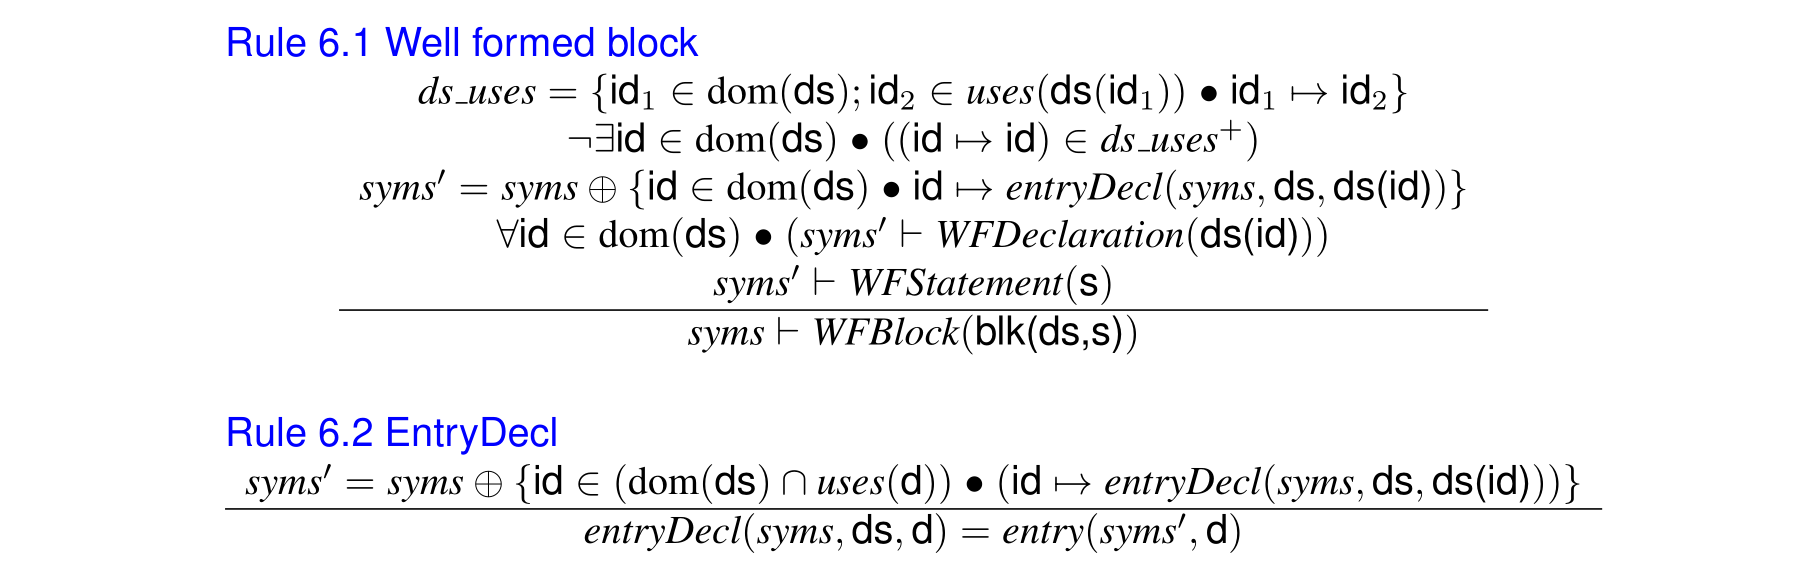
\includegraphics{assets/image-20200703193012243.png}

Intuitively, the predicate of rule 6.1 does the following:

\begin{itemize}
\tightlist
\item
  Constructs a mapping of identifiers to the identifiers they use and
  computes its transitive closure (denoted by superscript \(+\)).
\item
  Ensures that no identifier uses itself directly or indirectly,
  preventing recursion in the types.
\item
  Constructs a new scope \(\textit{syms}'\) by adding the new
  declarations and computing their symbol table entries using
  \(\textit{entryDecl}\) (discussed above).
\item
  Ensures that every new declaration is well-formed in the new context.
\item
  Ensures that in the new context, the statement list is well-formed.
\end{itemize}

If all of the above hold, the block as a whole is well-formed.

A \emph{program} is well-formed if its block is well-formed in the
context of the \(\textit{predefined}\) context.

\hypertarget{rules}{%
\subsection{Rules}\label{rules}}

\hypertarget{types-of-expressions}{%
\subsubsection{Types of Expressions}\label{types-of-expressions}}

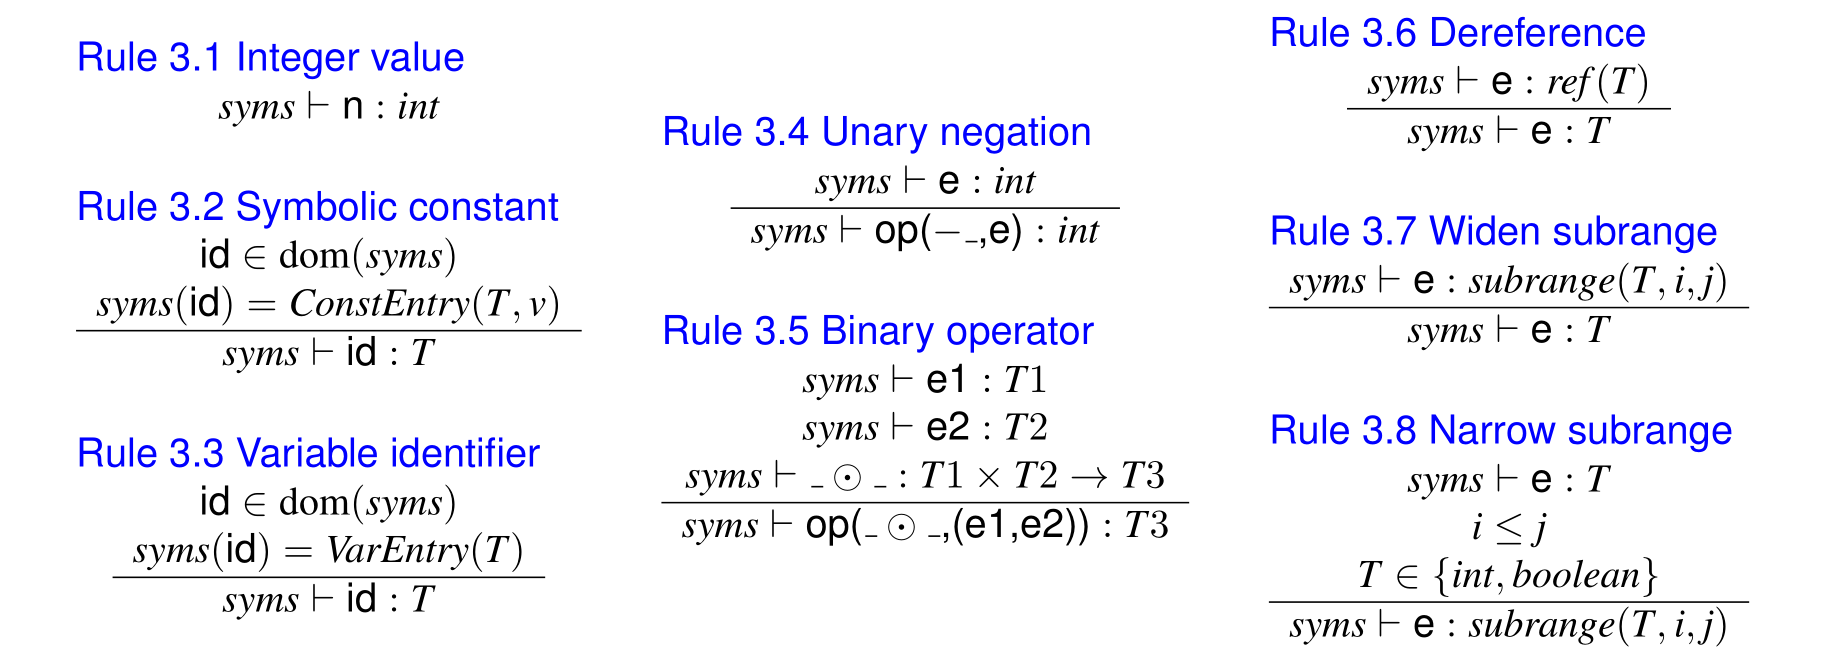
\includegraphics{assets/image-20200703200702094.png}

\hypertarget{well-formed-statements}{%
\subsubsection{Well-Formed Statements}\label{well-formed-statements}}

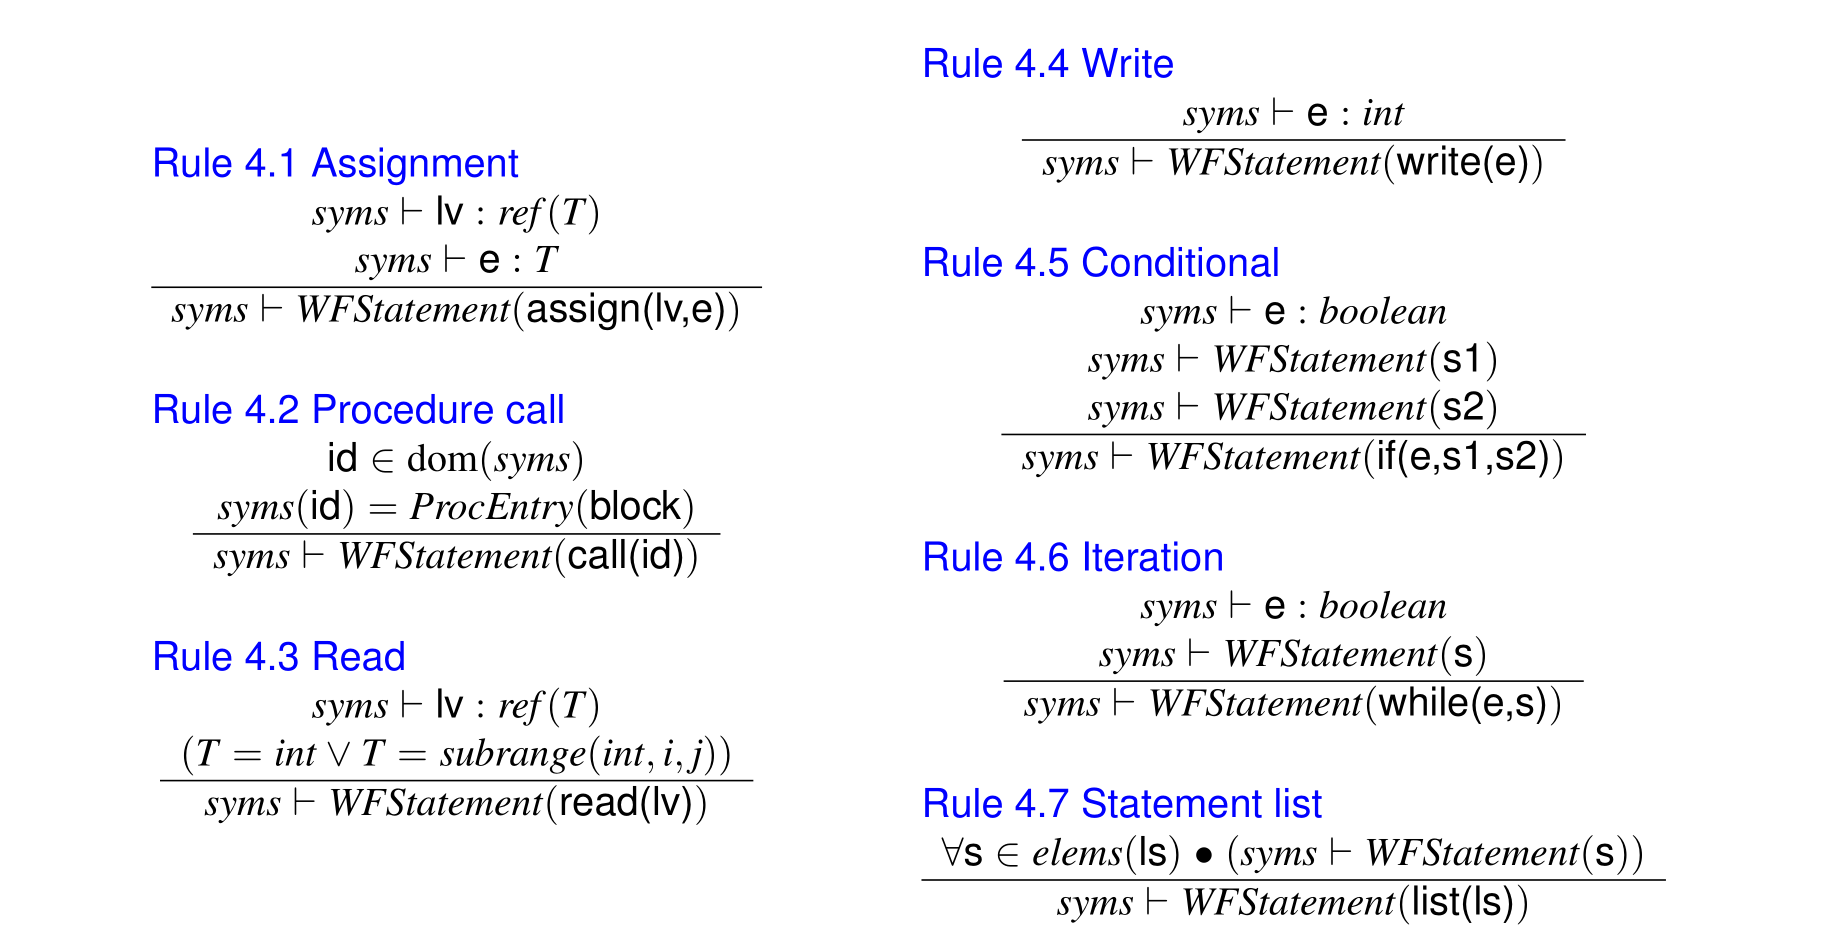
\includegraphics{assets/image-20200703200722065.png}

\hypertarget{well-formed-declarations}{%
\subsubsection{Well-Formed
Declarations}\label{well-formed-declarations}}

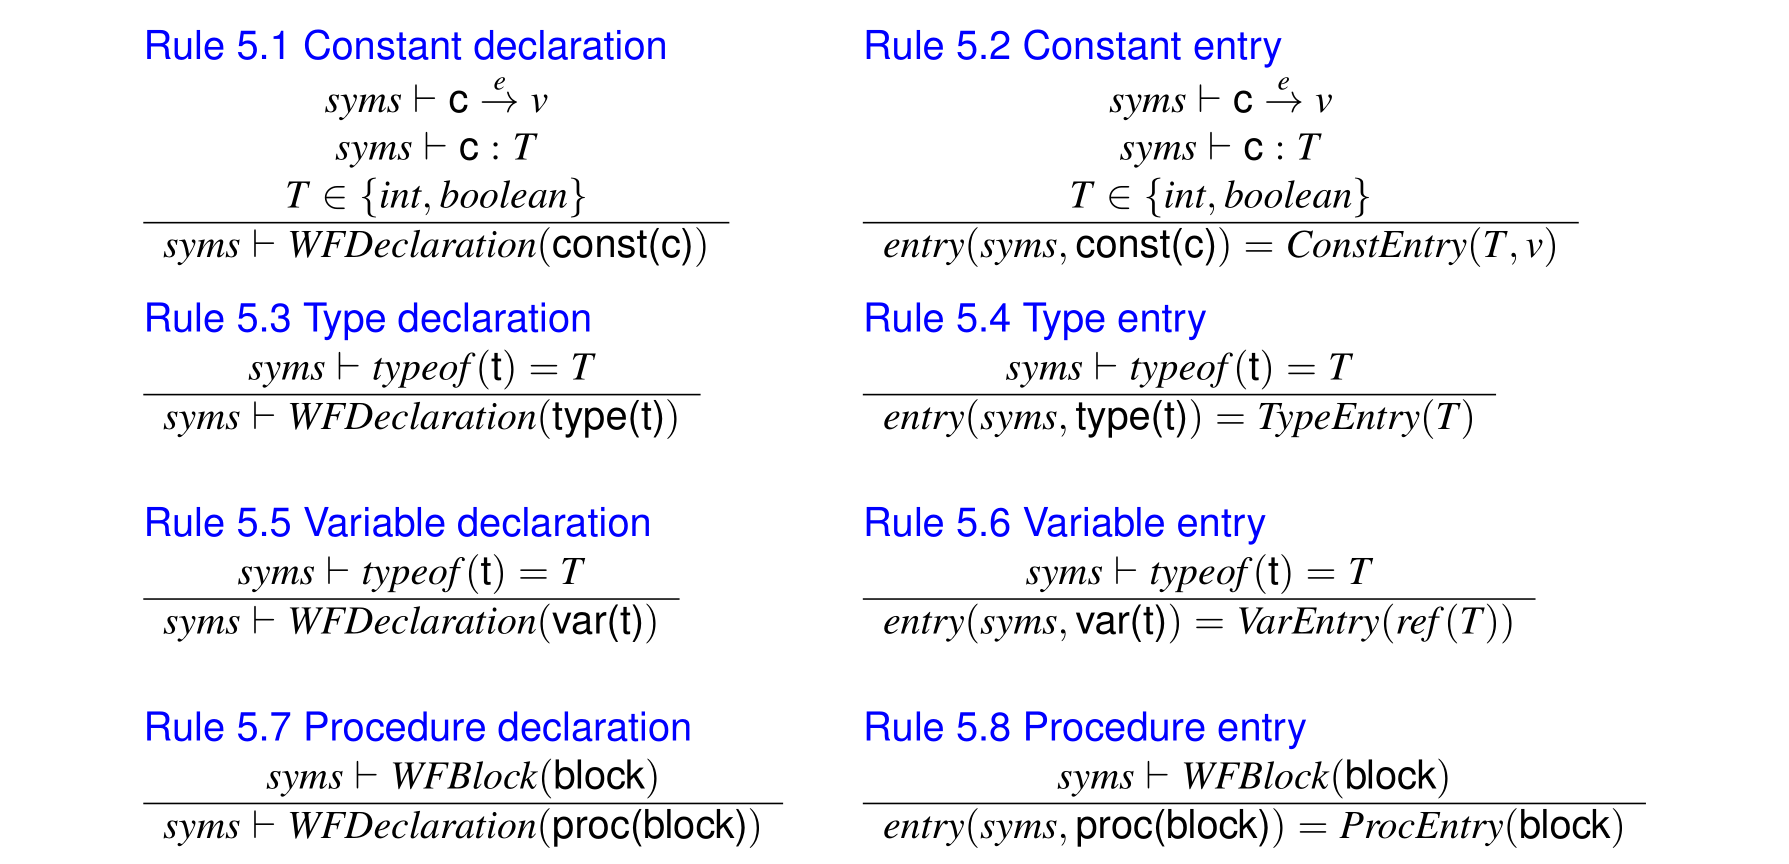
\includegraphics{assets/image-20200703200753360.png}

\hypertarget{constant-evaluation-rules}{%
\paragraph{Constant Evaluation Rules}\label{constant-evaluation-rules}}

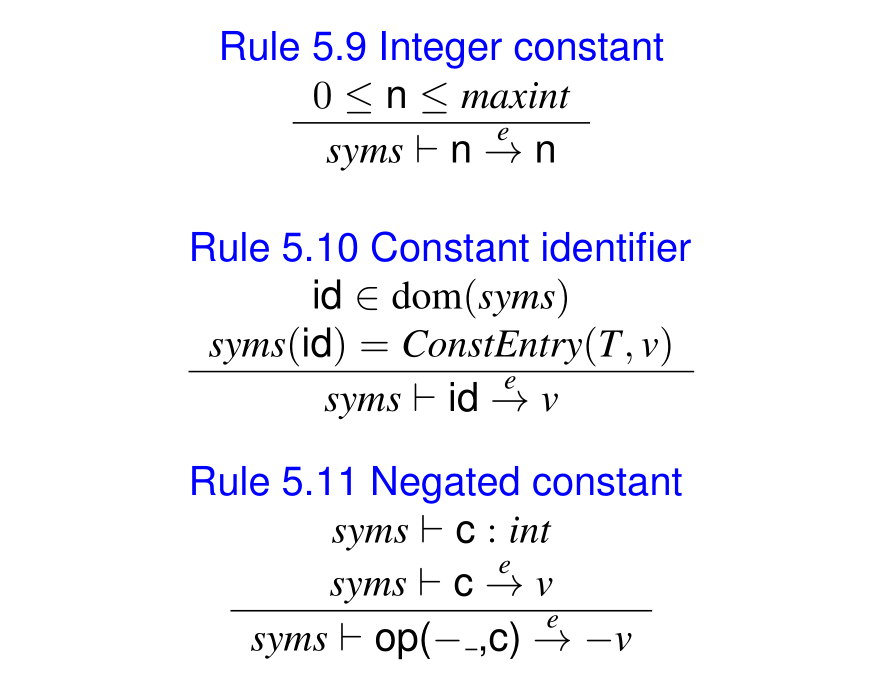
\includegraphics[width=0.5\textwidth]{assets/image-20200703200827441.png}

\hypertarget{well-formed-types}{%
\subsubsection{Well-Formed Types}\label{well-formed-types}}

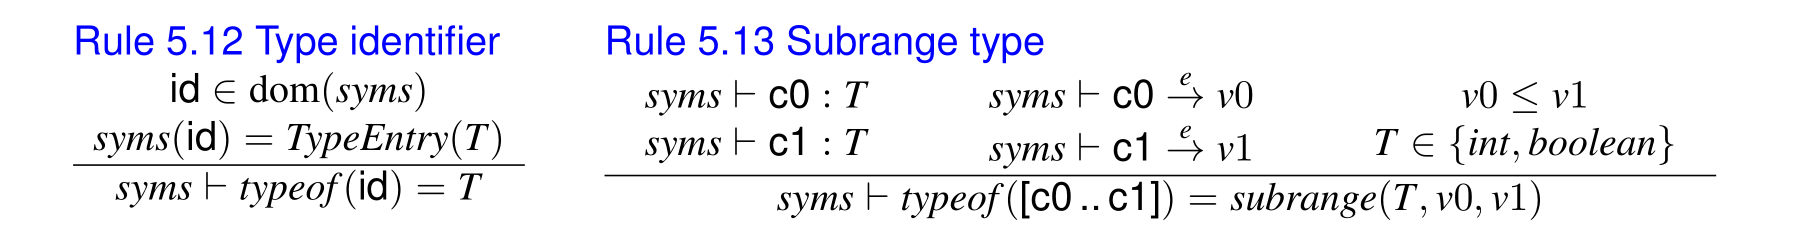
\includegraphics{assets/image-20200703200904388.png}

\hypertarget{well-formed-blocks}{%
\subsubsection{Well-Formed Blocks}\label{well-formed-blocks}}

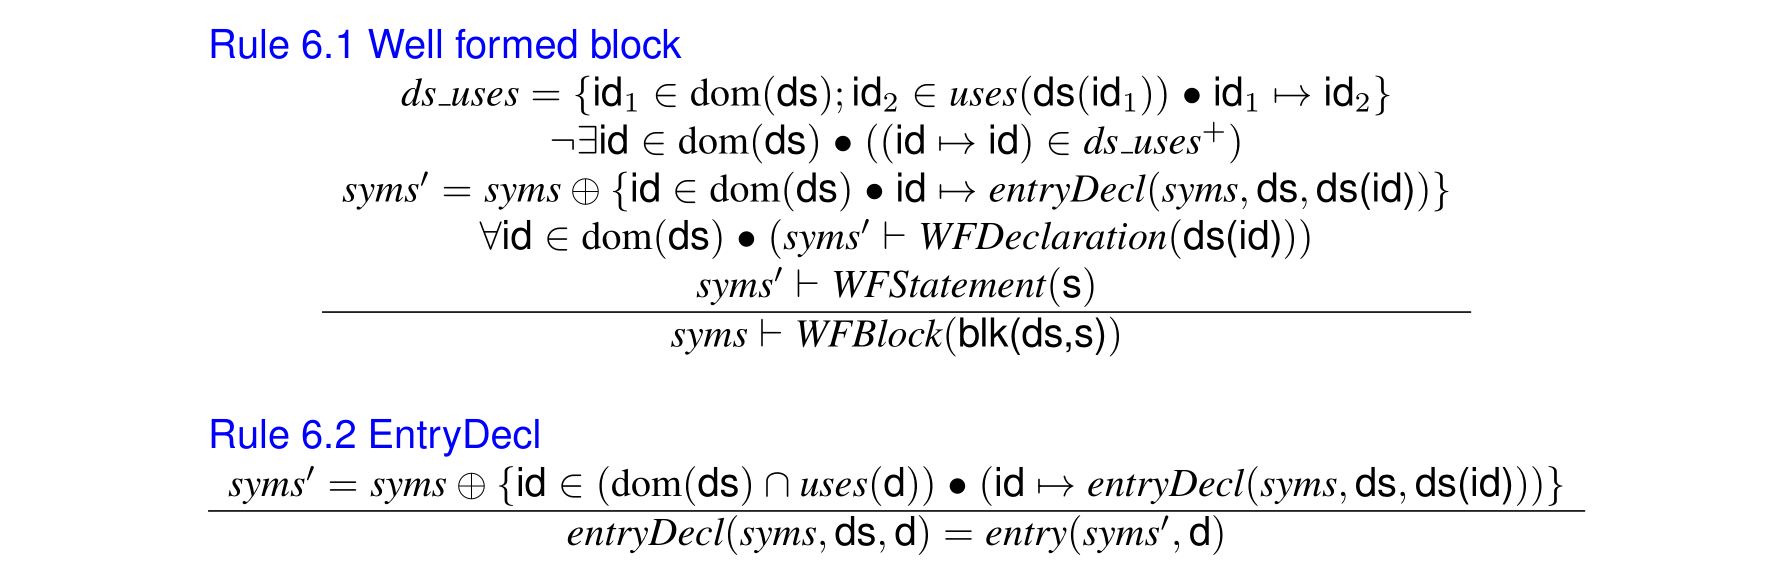
\includegraphics{assets/image-20200703200920326.png}

\hypertarget{well-formed-main-program}{%
\subsubsection{Well-Formed Main
Program}\label{well-formed-main-program}}

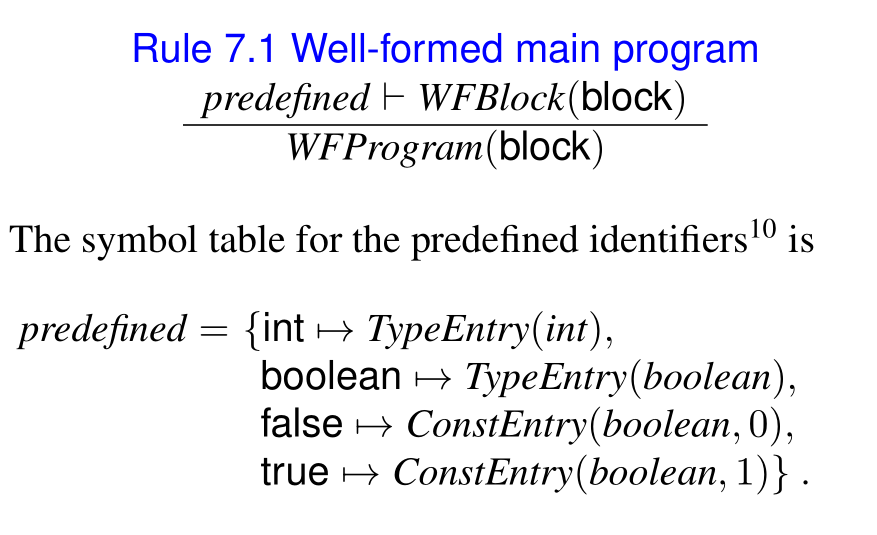
\includegraphics[width=0.5\textwidth]{assets/image-20200703200944338.png}

\end{document}
